% ============================================================
%  Manuscript v2: DNS Servers with BIND (revised after review of v1)
%  Build: latexmk   (see ./latexmkrc)   ->   build/main.pdf
%  Shared by all manuscript versions:  ../figures/  ../tables/
% ============================================================
\documentclass[10pt,letterpaper]{article}

\usepackage{arxiv}                 % vendored in docs/common/ (found via TEXINPUTS)
% ============================================================
%  Shared preamble for every LaTeX document in this repository.
%  Usage (after \usepackage{arxiv}):   % ============================================================
%  Shared preamble for every LaTeX document in this repository.
%  Usage (after \usepackage{arxiv}):   % ============================================================
%  Shared preamble for every LaTeX document in this repository.
%  Usage (after \usepackage{arxiv}):   \input{../../common/preamble}
%  Each document sets its own \graphicspath and \addbibresource.
% ============================================================

% ---------- Encoding, typography ----------
% No lmodern: arxiv.sty selects Times (ptm) as the roman family.
\usepackage[utf8]{inputenc}
\usepackage[T1]{fontenc}
\usepackage[english]{babel}
\usepackage{microtype}

% ---------- Tables, figures, code ----------
\usepackage{booktabs}
\usepackage{array}
\usepackage{tabularx}
\usepackage{graphicx}
\usepackage[table]{xcolor}
\usepackage{enumitem}
\usepackage{listings}

% Caption rules requested in the review (v1 feedback #1):
%   tables  -> caption ABOVE the table
%   figures -> caption below the figure
\usepackage{caption}
\captionsetup{font=small, labelfont=bf, labelsep=period}
\captionsetup[table]{position=top}
\captionsetup[figure]{position=bottom}

% ---------- Links and cross-references ----------
\usepackage{url}
\usepackage[hidelinks]{hyperref}
\usepackage[capitalise,noabbrev]{cleveref}
% Use \cref{fig:...}, \cref{tab:...}, \cref{sec:...} for EVERY float/section
% mention (never type "Figure 3" by hand; review feedback #3, #8).
\crefname{figure}{Figure}{Figures}
\crefname{table}{Table}{Tables}
\crefname{section}{Section}{Sections}
\crefname{subsection}{Section}{Sections}

% ---------- Bibliography (biblatex + biber, APA) ----------
\usepackage{csquotes}
\usepackage[style=apa, backend=biber]{biblatex}
\DeclareLanguageMapping{american}{american-apa}
% \addbibresource{...} is set in each main.tex (path depends on depth).

% ---------- Code listings ----------
\lstset{
  basicstyle=\ttfamily\footnotesize,
  backgroundcolor=\color{black!4},
  frame=single,
  rulecolor=\color{black!25},
  breaklines=true,
  columns=fullflexible,
  keepspaces=true,
  showstringspaces=false,
  xleftmargin=0.5em,
  xrightmargin=0.5em,
  aboveskip=0.8em,
  belowskip=0.8em,
}

% ---------- Helper macros ----------
% Pending item, visible in the draft (replaces Typst's #todo).
\newcommand{\todo}[1]{\textcolor{red}{\textbf{[TO DO: #1]}}}

% Unnumbered section that still appears in the table of contents.
% Use for "References" and "Declaration of AI Use" (review feedback #7).
\newcommand{\unnumberedsection}[1]{%
  \section*{#1}%
  \addcontentsline{toc}{section}{#1}%
}

% Inline code
\newcommand{\code}[1]{\texttt{#1}}

%  Each document sets its own \graphicspath and \addbibresource.
% ============================================================

% ---------- Encoding, typography ----------
% No lmodern: arxiv.sty selects Times (ptm) as the roman family.
\usepackage[utf8]{inputenc}
\usepackage[T1]{fontenc}
\usepackage[english]{babel}
\usepackage{microtype}

% ---------- Tables, figures, code ----------
\usepackage{booktabs}
\usepackage{array}
\usepackage{tabularx}
\usepackage{graphicx}
\usepackage[table]{xcolor}
\usepackage{enumitem}
\usepackage{listings}

% Caption rules requested in the review (v1 feedback #1):
%   tables  -> caption ABOVE the table
%   figures -> caption below the figure
\usepackage{caption}
\captionsetup{font=small, labelfont=bf, labelsep=period}
\captionsetup[table]{position=top}
\captionsetup[figure]{position=bottom}

% ---------- Links and cross-references ----------
\usepackage{url}
\usepackage[hidelinks]{hyperref}
\usepackage[capitalise,noabbrev]{cleveref}
% Use \cref{fig:...}, \cref{tab:...}, \cref{sec:...} for EVERY float/section
% mention (never type "Figure 3" by hand; review feedback #3, #8).
\crefname{figure}{Figure}{Figures}
\crefname{table}{Table}{Tables}
\crefname{section}{Section}{Sections}
\crefname{subsection}{Section}{Sections}

% ---------- Bibliography (biblatex + biber, APA) ----------
\usepackage{csquotes}
\usepackage[style=apa, backend=biber]{biblatex}
\DeclareLanguageMapping{american}{american-apa}
% \addbibresource{...} is set in each main.tex (path depends on depth).

% ---------- Code listings ----------
\lstset{
  basicstyle=\ttfamily\footnotesize,
  backgroundcolor=\color{black!4},
  frame=single,
  rulecolor=\color{black!25},
  breaklines=true,
  columns=fullflexible,
  keepspaces=true,
  showstringspaces=false,
  xleftmargin=0.5em,
  xrightmargin=0.5em,
  aboveskip=0.8em,
  belowskip=0.8em,
}

% ---------- Helper macros ----------
% Pending item, visible in the draft (replaces Typst's #todo).
\newcommand{\todo}[1]{\textcolor{red}{\textbf{[TO DO: #1]}}}

% Unnumbered section that still appears in the table of contents.
% Use for "References" and "Declaration of AI Use" (review feedback #7).
\newcommand{\unnumberedsection}[1]{%
  \section*{#1}%
  \addcontentsline{toc}{section}{#1}%
}

% Inline code
\newcommand{\code}[1]{\texttt{#1}}

%  Each document sets its own \graphicspath and \addbibresource.
% ============================================================

% ---------- Encoding, typography ----------
% No lmodern: arxiv.sty selects Times (ptm) as the roman family.
\usepackage[utf8]{inputenc}
\usepackage[T1]{fontenc}
\usepackage[english]{babel}
\usepackage{microtype}

% ---------- Tables, figures, code ----------
\usepackage{booktabs}
\usepackage{array}
\usepackage{tabularx}
\usepackage{graphicx}
\usepackage[table]{xcolor}
\usepackage{enumitem}
\usepackage{listings}

% Caption rules requested in the review (v1 feedback #1):
%   tables  -> caption ABOVE the table
%   figures -> caption below the figure
\usepackage{caption}
\captionsetup{font=small, labelfont=bf, labelsep=period}
\captionsetup[table]{position=top}
\captionsetup[figure]{position=bottom}

% ---------- Links and cross-references ----------
\usepackage{url}
\usepackage[hidelinks]{hyperref}
\usepackage[capitalise,noabbrev]{cleveref}
% Use \cref{fig:...}, \cref{tab:...}, \cref{sec:...} for EVERY float/section
% mention (never type "Figure 3" by hand; review feedback #3, #8).
\crefname{figure}{Figure}{Figures}
\crefname{table}{Table}{Tables}
\crefname{section}{Section}{Sections}
\crefname{subsection}{Section}{Sections}

% ---------- Bibliography (biblatex + biber, APA) ----------
\usepackage{csquotes}
\usepackage[style=apa, backend=biber]{biblatex}
\DeclareLanguageMapping{american}{american-apa}
% \addbibresource{...} is set in each main.tex (path depends on depth).

% ---------- Code listings ----------
\lstset{
  basicstyle=\ttfamily\footnotesize,
  backgroundcolor=\color{black!4},
  frame=single,
  rulecolor=\color{black!25},
  breaklines=true,
  columns=fullflexible,
  keepspaces=true,
  showstringspaces=false,
  xleftmargin=0.5em,
  xrightmargin=0.5em,
  aboveskip=0.8em,
  belowskip=0.8em,
}

% ---------- Helper macros ----------
% Pending item, visible in the draft (replaces Typst's #todo).
\newcommand{\todo}[1]{\textcolor{red}{\textbf{[TO DO: #1]}}}

% Unnumbered section that still appears in the table of contents.
% Use for "References" and "Declaration of AI Use" (review feedback #7).
\newcommand{\unnumberedsection}[1]{%
  \section*{#1}%
  \addcontentsline{toc}{section}{#1}%
}

% Inline code
\newcommand{\code}[1]{\texttt{#1}}
      % shared packages and macros

% ---------- Shared resources ----------
\graphicspath{{../figures/}}
\addbibresource{../../../bibliography.bib}

% ---------- Team data (edit) ----------
\newcommand{\teamname}{Team 1}
\newcommand{\coursename}{Applications of Cryptography and Cybersecurity}
\newcommand{\institution}{Tecnol\'ogico de Monterrey, Monterrey Campus}
\newcommand{\professor}{Mohd Anas Wajid}

\title{DNS Servers with BIND: Authoritative and Recursive Configuration, Root Hints, and Traffic Analysis}
\renewcommand{\headeright}{\teamname\ --- Technical report}
\renewcommand{\undertitle}{\coursename\ --- \institution}
\renewcommand{\shorttitle}{DNS Servers with BIND}

\author{%
  El\'ias Alejandro Corral Rodr\'iguez \\ A01743624
  \And
  Jannette Cristina Flores Rodr\'iguez \\ A01255711
  \And
  Angel Eduardo Luna \\ A00842657
  \And
  Montserrat Rodr\'iguez Ram\'irez \\ A01661271
  \And
  Carolina Sarah\'i S\'anchez Meneses \\ A00227980
}
\date{Professor: \professor \quad\textbullet\quad \today}

\hypersetup{pdftitle={DNS Servers with BIND}, pdfauthor={\teamname}}

\begin{document}
\maketitle

% Abstract + keywords (carried over from v1; revise if the findings changed)
\begin{abstract}
The goal of this activity is to study how DNS servers are configured with BIND, to distinguish authoritative from recursive servers, to understand the role of \code{root.hints}, and to analyze the structure of DNS responses with Wireshark and \code{dig}. The BIND and \code{root.hints} sections are theoretical, while the traffic analysis was carried out in practice on a real domain. This work is the foundation for a later lab in which DNSSEC will be implemented.
\end{abstract}
\keywords{DNS \and BIND \and Wireshark \and dig \and DNSSEC}

% \tableofcontents   % uncomment if the course requires a Contents page

\section{Introduction}\label{sec:introduction}

% TODO (feedback #2): every factual sentence ends with a citation.
% TODO (feedback #8): cite the environment table with \cref{tab:environment}.
% v1 source: Introduction (3 paragraphs), Objectives, Environment table.

\subsection{Objectives}\label{sec:objectives}

\subsection{Environment used for the traffic analysis}\label{sec:environment}
% Table caption goes ABOVE the table (handled by the shared preamble).
% Values captured on the lab machines need a source figure (feedback #4):
%   "Source: \cref{fig:...}" in the table notes.

\section{What Is BIND and How Is It Used in DNS?}\label{sec:bind}

% v1 source: Section 2 (Overview, Main functions table).
% TODO (feedback #2): cite BIND history/tools; (#8) cite the functions table.

\subsection{Overview}\label{sec:bind-overview}

\subsection{Main functions}\label{sec:bind-functions}

\section{BIND Configuration Options}\label{sec:configuration}

% v1 source: Section 3 (files table, authoritative, recursive, comparison, verification).
% TODO (feedback #2): the allow-recursion / open-resolver / amplification claims need sources.
% TODO (feedback #8): cite every table and the code listings in the text.

\subsection{Configuration files involved}\label{sec:config-files}

\subsection{Authoritative server}\label{sec:config-authoritative}

\subsection{Recursive server}\label{sec:config-recursive}

\subsection{Authoritative vs.\ recursive comparison}\label{sec:config-comparison}

\subsection{Configuration verification}\label{sec:config-verification}

\section{Importance of the \code{root.hints} File}\label{sec:root-hints}

% v1 source: Section 4.
% TODO (feedback #2): cite the built-in-hints claim and the IANA source.

\subsection{Role in iterative resolution}\label{sec:root-hints-role}

\section{DNS Query Analysis with Wireshark and \code{dig}}\label{sec:analysis}

% v1 source: Section 5 (methodology, response sections, SOA, NS, A, AAAA, TTL summary).
% Rules for this section (review feedback):
%   #3/#8  every screenshot is a labelled figure and is mentioned with \cref{fig:...}
%          next to the values it supports
%   #5     use the highlighted screenshots (see docs/action-plan notes)
%   #4     each table built from captures cites its source figure(s)
%   #2     RFC-defined behaviour (flags, EDNS, TTL, negative caching) carries a citation

\subsection{Methodology}\label{sec:methodology}

\subsection{Sections of a DNS response message}\label{sec:response-sections}

\subsection{SOA records}\label{sec:soa}

\subsection{NS records}\label{sec:ns}

\subsection{A records}\label{sec:a}

\subsection{AAAA records}\label{sec:aaaa}

\subsection{TTL summary by record}\label{sec:ttl}

% ------------------------------------------------------------
% SMOKE TEST: proves the shared ../figures, ../tables and the
% bibliography work. Delete this block when real content is in.
% ------------------------------------------------------------
\paragraph{Smoke test.}
The captured packets are shown in \cref{fig:capture-overview}; their TTL values are
summarized in \cref{tab:example} \parencite{rfc1035}.

\begin{figure}[htbp]
  \centering
  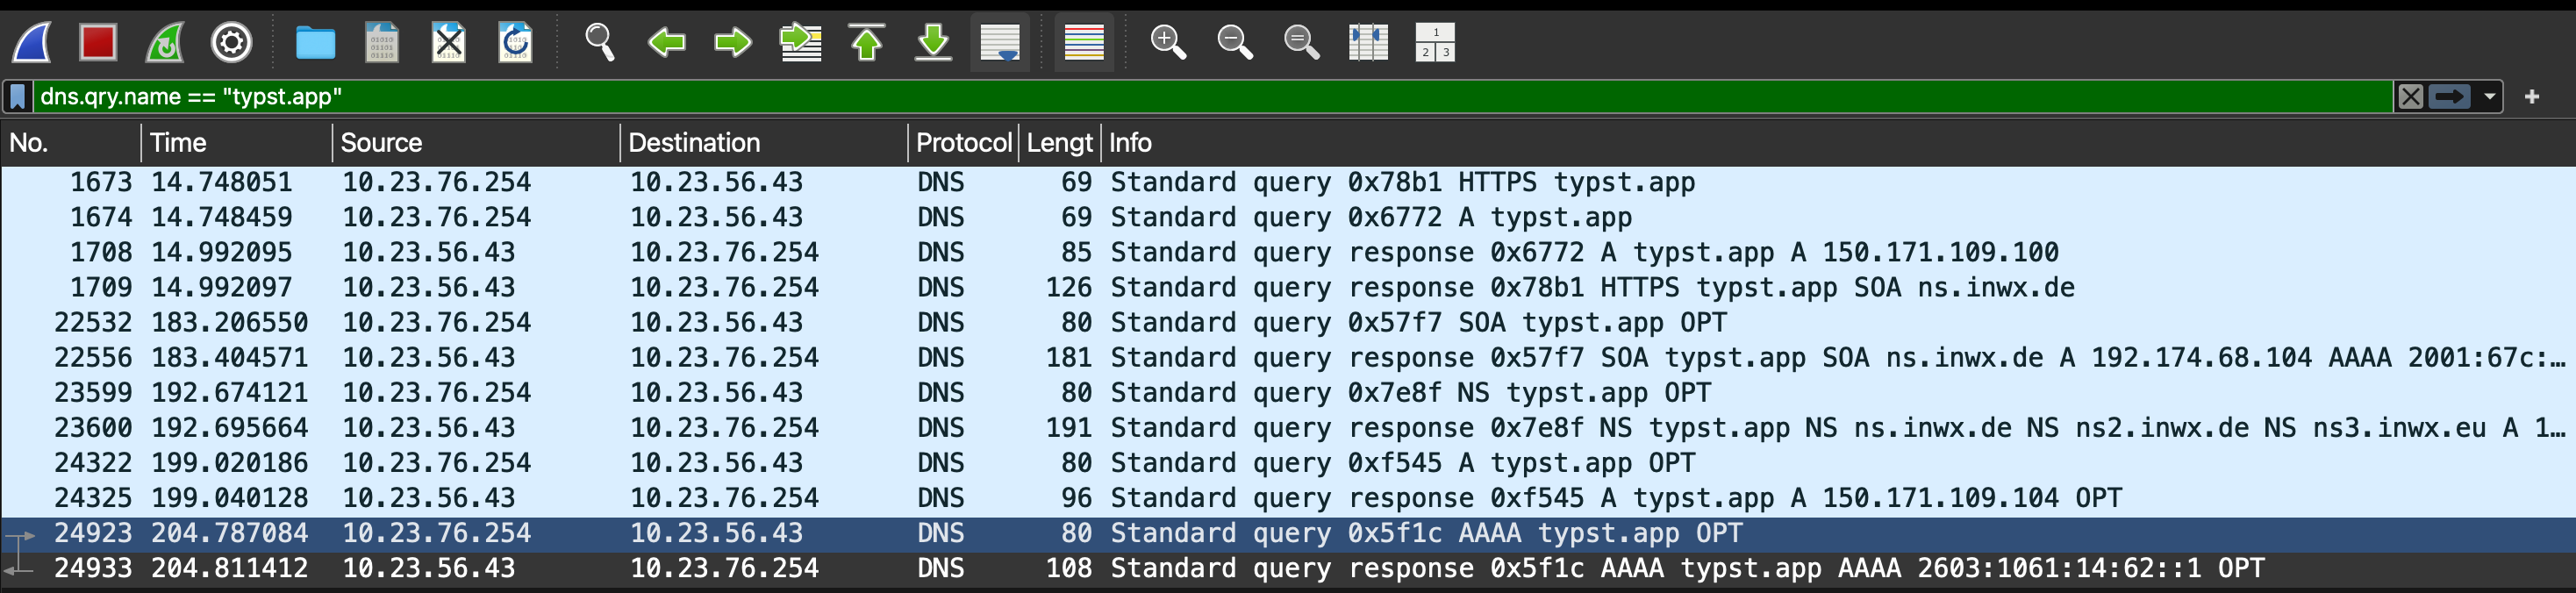
\includegraphics[width=\linewidth]{real dig typst.png}
  \caption{DNS packets for \code{typst.app} captured on Wi-Fi (\code{en0}) with the filter \code{dns.qry.name == "typst.app"}.}
  \label{fig:capture-overview}
\end{figure}

% Example shared table fragment. Include with % Example shared table fragment. Include with \input{../tables/tab-example}
% (from docs/manuscript/vN/sections/*.tex).  Delete once real tables exist.
% Conventions: caption ABOVE (booktabs, no vertical rules), \label{tab:...},
% and a "Source" note naming the figure the values come from.
\begin{table}[htbp]
  \centering
  \caption{Observed TTL for each record type in \code{typst.app} (example fragment).}
  \label{tab:example}
  \begin{tabular}{@{}llr@{}}
    \toprule
    Type & Name & TTL (s) \\
    \midrule
    NS   & \code{typst.app.} & 4076 \\
    A    & \code{typst.app.} & 300  \\
    \bottomrule
  \end{tabular}

  \smallskip
  \footnotesize Source: \cref{fig:capture-overview}.
\end{table}

% (from docs/manuscript/vN/sections/*.tex).  Delete once real tables exist.
% Conventions: caption ABOVE (booktabs, no vertical rules), \label{tab:...},
% and a "Source" note naming the figure the values come from.
\begin{table}[htbp]
  \centering
  \caption{Observed TTL for each record type in \code{typst.app} (example fragment).}
  \label{tab:example}
  \begin{tabular}{@{}llr@{}}
    \toprule
    Type & Name & TTL (s) \\
    \midrule
    NS   & \code{typst.app.} & 4076 \\
    A    & \code{typst.app.} & 300  \\
    \bottomrule
  \end{tabular}

  \smallskip
  \footnotesize Source: \cref{fig:capture-overview}.
\end{table}


\section{Results and Discussion}\label{sec:results}

% v1 source: Section 6 (auth vs recursive, root.hints effect, response analysis, TTL behaviour).
% TODO (feedback #2): v1 had NO citations here; restate each claim with its citation.
% TODO (feedback #4/#8): the sections-summary table cites its source figure.

\subsection{Authoritative vs.\ recursive servers}\label{sec:res-auth-rec}

\subsection{Effect of \code{root.hints}}\label{sec:res-root-hints}

\subsection{Analysis of the DNS response}\label{sec:res-response}

\subsection{TTL behavior}\label{sec:res-ttl}

\section{Conclusions}\label{sec:conclusions}

% TODO (feedback #6): write in PARAGRAPHS, not a numbered list.
% Draft proposal: docs/action-plan/05-conclusions.md (Typst syntax; translate @key -> \parencite{key}, @fig-x -> \cref{fig:x}).
% Keep citations and figure references for every restated finding.

% Unnumbered (feedback #7), but listed in the table of contents.
\printbibliography[heading=bibintoc, title={References}]
         % unnumbered
% Unnumbered (feedback #7), but listed in the table of contents.
\unnumberedsection{Declaration of AI Use}

\todo{Update the v1 declaration: tools used, dates (v1: November 6--9, 2026), what they were used for, and what the team verified. Cite the model with \texttt{\textbackslash parencite\{anthropic2026sonnet55\}}.}
     % unnumbered

\end{document}
